\documentclass[11pt,letterpaper]{article}
\usepackage[lmargin=1in,rmargin=1in,tmargin=1in,bmargin=1in]{geometry}
\usepackage{../style/homework}
\setbool{quotetype}{false} % True: Side; False: Under
\setbool{hideans}{true} % Student: True; Instructor: False

\usepackage{float} % Force Table Placement

% -------------------
% Content
% -------------------
\begin{document}

\homework{9: Due 02/28}{[Penny] God, you know, four years I lived with him. Four years---that's like as long as high school. [Sheldon] It took you four years to get through high school?}{Penny \& Sheldon Cooper, Big Bang Theory}

% Problem 1
\problem{10} Determine whether the relations $F$ and $G$ shown below are functions. Be sure to fully justify your answer. \pspace
	\hfill
	\begin{minipage}[c]{0.48\textwidth}
	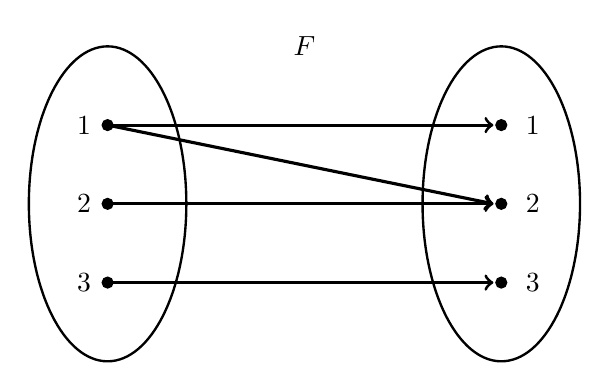
\begin{tikzpicture}
	\node at (2.5,2) {$F$};
	% Ellipses
	\draw[line width=0.03cm] (0,0) circle (1 and 2);
	\draw[line width=0.03cm] (5,0) circle (1 and 2);
	
	% Nodes
	\draw[fill=black] (0,1) circle (0.07);
	\draw[fill=black] (0,0) circle (0.07);
	\draw[fill=black] (0,-1) circle (0.07);
	
	\draw[fill=black] (5,1) circle (0.07);
	\draw[fill=black] (5,0) circle (0.07);
	\draw[fill=black] (5,-1) circle (0.07);
	
	% Arrow
	\draw[line width=0.04cm,->] (0,1) -- (4.9,1);
	\draw[line width=0.04cm,->] (0,1) -- (4.9,0);
	\draw[line width=0.04cm,->] (0,0) -- (4.9,0);
	\draw[line width=0.04cm,->] (0,-1) -- (4.9,-1);
	
	% Labels
	\node at (-0.3,1) {$1$};
	\node at (-0.3,0) {$2$};
	\node at (-0.3,-1) {$3$};
	
	\node at (5.4,1) {$1$};
	\node at (5.4,0) {$2$};
	\node at (5.4,-1) {$3$};
	\end{tikzpicture}
	\end{minipage}%
	\begin{minipage}[c]{0.40\textwidth}
	\begin{table}[H]
	\centering
	\begin{tabular}{cc}
	$x$ & $G$ \\ \hline
	$1$ & $1$ \\
	$2$ & $1$ \\
	$3$ & $1$ \\
	$4$ & $1$ \\
	$5$ & $1$
	\end{tabular}
	\end{table}
	\end{minipage} 



\newpage



% Problem 2
\problem{10} Determine whether the relations $f(x)= 16 - x^2$ and $g(x, y)= \dfrac{x + y}{x - y}$ are functions. Be sure to fully justify your answer. Also, find $f(5)$ and $g(4, 5)$. 



\newpage



% Problem 3
\problem{10} Suppose $f(x)$ and $g(x)$ are the functions given below. 
	\[
	\begin{aligned}
	f(x)&= 1 - 4x \\[0.3cm]
	g(x)&= x^2 + 1
	\end{aligned}
	\]

Compute the following: \pspace
        \begin{enumerate}[(a)]
        \item $6f(1) - g(2)$ \vfill
        \item $(f + g)(1)$ \vfill
        \item $(f - g)(0)$ \vfill
        \item $(fg)(2)$ \vfill
        \item $(f \circ g)(-1)$ \vfill
        \item $(g \circ f)(-1)$ \vfill
        \end{enumerate} 


\end{document}